\documentclass[12pt,a4paper]{article}
%%%%%%%%%% pacotes
\usepackage{amsmath,amsfonts,amssymb}
\usepackage[portuguese]{babel}
\usepackage[dvipsnames]{xcolor}
\usepackage[left=2cm,right=2cm,top=2cm,bottom=2cm]{geometry}
\usepackage{
    txfonts,
    %cancel,
    hyperref,
    graphicx,
    float,
}

%%%%%%%%%% configs
\title{Multi Layer Perceptron\\MLP}
\author{Junior R. Ribeiro \\ \url{jrodrib@usp.br}}
\date{\today}
\hypersetup{
    colorlinks=true,
    linkcolor=blue,
    filecolor=magenta,
    urlcolor=cyan,
}
\setlength{\parskip}{12pt}
\setlength{\parindent}{12pt}

%%%%%%%%%% comandos
\def\RR{\mathbb{R}}
\def\bfE{\mathbf{E}}

\DeclareMathOperator{\logistic}{logistic}
\begin{document}

\maketitle\tableofcontents

\section{Multicamadas}

Considere as camadas $\ell=0,...,L$ em que os neurônios de uma camada somente se comunicam com os neurônios em camadas vizinhas. Quando isso acontece, dizemos que o MLP é sem atalhos.

Considere os padrões de entrada $\bar x(n)\in\RR^{m_0-1}$ para cada $n=0,...,N-1$ (um total de $N$ padrões de entrada), com suas respectivas saídas desejadas $d(n)\in\Omega^{m_L}$ em que $\Omega=[0,1]$ ou $\Omega=[-1,1]$, dependendo do problema. As camadas $\ell=0$ e $\ell=L$ são as camadas de entrada e saída da rede, e todas as camadas $0<\ell<L$ são camadas ocultas.

As dimensões das variáveis usadas para cômputo do fluxo da rede são $m_0, m_1,...,m_L$. Por causa dos \textit{biases} as variáveis do fluxo principal entre os neurônios (exceto os \textit{biases}) têm dimensões $m_0-1, m_1-1,...,m_{L-1}-1,m_L$, pois na camada de saída não há \textit{bias} (note a dimensão de $d(n)$)

As variáveis que efetuam o fluxo da rede são $y^\ell$ para cada camada $\ell=0,...,L$ (os superíndices indicam a camada em questão). Essas variáveis representam o valor de saída de cada nó.

\subsection{Esboço do fluxo}
Todos os índices neste texto foram pensados como iniciando em zero. Destacamos em {\color{purple} roxo} as principais partes para implementação.

$\color{purple}
y^0(n) = \begin{bmatrix}
1\\
\bar x_0(n)\\
:\\
\bar x_{m_0-2}(n)
\end{bmatrix}
=:
\begin{bmatrix}
	1\\
	v_0^0(n)\\
	:\\
	v_{m_0-2}^0(n)
\end{bmatrix}
\in \RR^{m_0}
$

\noindent e para as diversas camadas $\ell=0,...,L-1$, temos


$\color{purple}
w^\ell = \begin{bmatrix}
	b_0^\ell & W_{0,0}^\ell & .. & W_{0,m_\ell-2}^\ell\\
	:\\
	b_{m_{\ell+1}-2}^\ell & W_{m_{\ell+1}-2,0}^\ell & .. & W_{m_{\ell+1}-2,m_\ell-2}^\ell\\
\end{bmatrix}
\in \RR^{(m_{\ell+1}-1)\times m_\ell};
$


$\color{purple}
v^{\ell+1}(n) = 
\begin{bmatrix}
v^{\ell+1}_0(n)\\
:\\
v^{\ell+1}_{m_{\ell+1}-2}(n)
\end{bmatrix}
=w^\ell y^\ell(n)=
\begin{bmatrix}
	b_0^\ell & W_{0,0}^\ell & .. & W_{0,m_\ell-2}^\ell\\
	:\\
	b_{m_{\ell+1}-2}^\ell & W_{m_{\ell+1}-2,0}^\ell & .. & W_{m_{\ell+1}-2,m_\ell-2}^\ell\\
\end{bmatrix}
\begin{bmatrix}
	1\\
	 v_0^\ell(n)\\
	:\\
	 v_{m_\ell-2}^\ell(n)
\end{bmatrix}
\in \RR^{(m_{\ell+1}-1)},
$
 


$\color{purple}
y^{\ell}(n) = \begin{bmatrix}
	1\\
	\logistic(v_0^{\ell}(n))\\
	:\\
	\logistic(v_{m_{\ell}-2}^{\ell}(n))
\end{bmatrix}
\in \RR^{m_{\ell+1}};
$

\noindent e por fim (não tem \textit{bias} na camada de saída)

$\color{purple}
y^L(n) = \begin{bmatrix}
	\varphi(v_0^L(n))\\
	:\\
	\varphi(v_{m_L-1}^L(n))
\end{bmatrix}
\in \RR^{m_L}
$

Para cada problema (classificação, regressão), usamos uma função $\varphi(\cdot)$ diferenciada. As variáveis $w^\ell=[b^\ell\;\;W^\ell]$ são os pesos da rede entre as camadas $\ell=0,...,L-1$.


\noindent Temos o erro

$
e_k(n) = d_k(n) - y^L_k(n), \qquad k=0,...,m_L-1.
$

ou vetorialmente,

$\color{purple}
e(n) = d(n)-y(n) \in\RR^{m_L},
$

\noindent e o erro quadrático acumulado

$
\displaystyle E(n) = 0.5\sum_{k=0}^{m_L-1}e_k^2(n).
$

ou vetorialmente

$\color{purple}
E(n) = 0.5e(n)^Te(n) \in\RR
$








\section{Gradiente}
Considere os nós $i$ na camada $L-2$, $j$ na camada $L-1$ e $k$ na camada $L$. Vamos derivar o erro quadrático acumulado em relação aos pesos ajustáveis $w^{L-1}$. Como a dependência entre essa svariáveis não é direta, aplicamos a regra da cadeia.

A Figura \ref{fig:rede} ilustra em laranjado $w_{kj}^{L-1}$ para $k=0$ e $j=2$. Note que o erro $E$ depende de $w_{02}^{L-1}$ apenas através de uma única parcela que consta no nó $k=0$.

\noindent Esquema:

$
\begin{matrix}
	\mbox{camada}\rightarrow\\
	\mbox{fluxo}\rightarrow
\end{matrix}\;\;
\begin{pmatrix}
	L-1 & L-1 & L &&L&&d_k\downarrow\\
	y_j & \stackrel{w_{kj}}{\longrightarrow}&
	v_k & \stackrel{\varphi}{\longrightarrow}&y_k&
	\stackrel{-1}{\longrightarrow}& e_k
\end{pmatrix}
$

\noindent Conforme visto no esquema acima, fazemos

$
\dfrac{\partial E(n)}{\partial w_{kj}^{L-1}}
=
\dfrac{\partial E(n)}{\partial e_k(n)}
\;
\dfrac{\partial e_k(n)}{\partial y^{L}_k(n)}
\;
\dfrac{\partial y^L_k(n)}{\partial v_k^{L}(n)}
\;
\dfrac{\partial v_k^L(n)}{\partial w^{L-1}_{kj}}
=
e_k(n) \cdot (-1) \cdot \varphi'(v_k^L(n)) \cdot y^{L-1}_j(n)
$

\noindent Vamos definir o produto ``ponto-a-ponto'' entre matrizes de mesma dimensão, como sendo

$
[A\bullet B]_{ij} = A_{ij}B_{ij}.
$



Defina

\begin{equation}\label{delta-1}
\delta^{L-1}_k(n) = -\dfrac{\partial E(n)}{\partial v^L_k(n)} = e_k(n) \varphi'(v_k^L(n))  
, \quad k=0,...,m_L-1,
\end{equation}

ou vetorialmente

\begin{itemize}\color{purple}
\item quando $\varphi(z)=\logistic(z)$,
\[
\delta^{L-1}(n) = e(n)\bullet \logistic(v^L(n))\bullet \Big(\mathbf{1}-\logistic(v^{L}(n))\Big);
\]
\item quando $\varphi(z)=z$,
\[
\delta^{L-1}(n) = e(n);
\]
\item quando $\varphi(z)=\tanh(z)$,
\[
\delta^{L-1}(n) = e(n)\bullet \Big(\mathbf{1}-\tanh(v^L(n))\bullet \tanh(v^L(n))\Big).
\]
\end{itemize}


Com essa definição, podemos escrever

\begin{equation}
\dfrac{\partial E(n)}{\partial w^{L-1}_{kj}} = -\delta^{L-1}_k(n) y_j^{L-1}(n), \quad k=0,...,m_L-1.
\end{equation}


\begin{figure}[H]\centering
	\label{fig:rede}
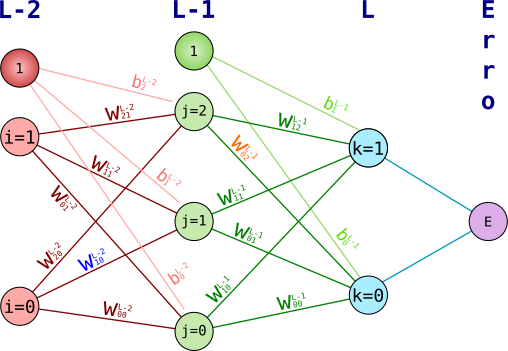
\includegraphics[width=0.7\textwidth]{rede}
\caption{Camadas $\ell=L-2,L-1,L$ e o erro $E(n)$. Os pesos $w^{L-2}_{10}$ e $w^{L-1}_{02}$ foram destacados.}
\end{figure}


Para calcular a taxa de variação de $E(n)$ em relação a $w^{L-2}_{ji}$, precisamos seguir o fluxo na rede no sentido ``do final para o começo'' ou \textit{backward}. Portanto, note que precisamos fazer um somatório, pois as parcelas de todos os nós $k$ são alteradas quando alteramos $w^{L-2}_{ji}$, o que não acontecia na situação anterior.  

$
\begin{aligned}
\dfrac{\partial E(n)}{\partial w^{L-2}_{ji}} 
&= \displaystyle\sum_{k=0}^{m_L-1}
\dfrac{\partial E(n)}{\partial e_k(n)}
\;
\dfrac{\partial e_k(n)}{\partial y^{L}_k(n)}
\;
\dfrac{\partial y^L_k(n)}{\partial v_k^{L}(n)}
\;
\dfrac{\partial v_k^L(n)}{\partial y^{L-1}_{j}(n)}
\;
\dfrac{\partial y^{L-1}_{j}(n)}{\partial v^{L-1}_{j}(n)}
\;
\dfrac{\partial v^{L-1}_{j}(n)}{\partial w^{L-2}_{ji}}
\\
&=\displaystyle\sum_{k=0}^{m_L-1}
e_k(n) \cdot (-1) \cdot
\varphi'(v_k^{L}(n)) \cdot w_{kj}^{L-1} \cdot \logistic'(v_j^{L-1}(n)) \cdot y_i^{L-2}(n)
\\
&=\displaystyle-\logistic'(v_j^{L-1}(n)) \cdot y_i^{L-2}(n)\sum_{k=0}^{m_L-1}
\underbrace{e_k(n) \cdot  
\varphi'(v_k^{L}(n))}_{\delta^{L-1}_k(n)} \cdot w_{kj}^{L-1} 
\\
&=\displaystyle-\logistic'(v_j^{L-1}(n))   y_i^{L-2}(n)\sum_{k=0}^{m_L-1}
\delta^{L-1}_k(n)  w_{kj}^{L-1} .
\end{aligned}
$

Defina

\begin{equation}\label{delta:}
\delta^{L-2}_j(n)
=
-\dfrac{\partial E(n)}{\partial v_j^{L-1}(n)}
=\displaystyle
 \logistic'(v_j^{L-1}(n))   \sum_{k=0}^{m_L-1}
\delta^{L-1}_k(n)  w_{kj}^{L-1} 
, \quad j=0,...,m_{L-1}-1,
\end{equation}

ou vetorialmente, para a camada $\ell=0,...,L-2$,
\[\color{purple}
\delta^{\ell}(n)= \Bigg[
\logistic(v^{\ell+1}(n))
\bullet
	\Big(
	\mathbf{1}-\logistic(v^{\ell+1}(n))
	\Big)
\Bigg]
\bullet \Big[(w^{\ell+1})^T\delta^{\ell+1}(n)\Big].
\]


Com essa definição, escrevemos

\begin{equation}
\dfrac{\partial E(n)}{\partial w^{L-2}_{ji}}
=
-\delta^{L-2}_j(n)y_i^{L-2}(n)
, \quad j=0,...,m_{L-1}-1 .
\end{equation}


O gradiente do erro em relação aos pesos, ou seja, a derivada de primeira ordem da função erro $E(n)$ em relação a cada $w_{rs}^\ell$ de cada camada $\ell=0,...,L-1$ é a coleção de matrizes $w^{\ell}$. Perceba que não é um vetor, nem uma matriz, mas uma coleção de matrizes.

\subsection{Direção de descida}
Em um método de minimização de primeira ordem, a ideia principal é caminhar na direção oposta à do gradiente. Portanto, o incremento $\Delta w_\rho(n)$ da iteração/ciclo $\rho$ que atualiza cada um dos pesos $w$, na forma $\color{purple}w^\ell_{\rho+1}\gets w^\ell_{\rho}+ \Delta w^\ell_\rho(n)$, com tamanho de passo $0<\eta\le1$ é dado por

\begin{equation}
\Delta w^{\ell}_{sr}(n) = \eta \delta_s^{\ell}(n)y_r^{\ell}(n),
\quad r=0,...,m_{\ell}-1 
\quad s=0,...,m_{\ell+1}-1,
\quad \ell=0,...,L-1,
\end{equation}

ou vetorialmente, para $\ell=0,...,L-1$

$\color{purple}
\Delta w^\ell_\rho(n) = \eta\delta^\ell(n)(y^\ell(n))^T.
$

Se quisermos adicionar Momentum, precisamos armazenar $\Delta w^\ell_{\rho-1}(n)$ da iteração $\rho-1$ e dar uma constante $0<\alpha<1$ com 

$\color{purple}
\Delta w^\ell_\rho(n) = \eta\delta^\ell(n)(y^\ell(n))^T
+\alpha \Delta w^\ell_{\rho-1}(n).
$

O termo Momentum nada mais é do que o gradiente da iteração anterior. Para inicializar o termo Momentum, comece-o em zero.

\begin{figure}[H]\centering
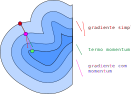
\includegraphics[width=0.6\textwidth]{momentum}
\caption{Ilustração do termo Momentum afetando a direção de descida.}
\end{figure}



\section{Função de ativação}
Em problemas de regressão segundo \cite{riedmiller}, usamos uma função linear, $\varphi(z)=z$ e portanto a derivada é a função constante $\varphi'(z)=1$, vide equação \eqref{delta-1}.

Em problemas de classificação, usamos $\varphi(z)=\logistic(z)$, uma função com imagem $(0,1)$:

$
\logistic(z) = \dfrac{1}{1+\exp(-z)}
$

$
\logistic'(z) = \logistic(z)(1-\logistic(z))
$, vide equações \eqref{delta-1} e \eqref{delta:}.


Uma alternativa à função logística é usar $\varphi(z)=\tanh(z)$, uma função com imagem $(-1,1)$:

$
\tanh(z) = \dfrac{\exp(2z)-1}{\exp(2z)+1}
$

$
\tanh'(z) = 1 - \tanh^2(z)
$, vide equações \eqref{delta-1} e \eqref{delta:}.


\section{Modo cíclico}
Agora que já sabemos como calcular o erro $E$ e as taxas de variação de $E$ em função de $w$ em todas as camadas, podemos aplicar qualquer método de minimização de primeira ordem. Na seção ``Direção de descida'' é dado um método com tamanho de passo fixo $\eta$, mas podemos fazer inúmeras variações de algoritmo de forma a torná-lo adaptativo, ou mesmo estocástico. Escrevendo o problema de otimização, temos
\[
\underset{W}{\mbox{minimizar }} E(W,n),
\]
\[
 W=\big\{w^\ell_{i,j}
 \quad i=0,...,m_{\ell+1}-1, \quad j=0,...,m_\ell-1,\quad \ell=0,...,L-1
\big\}
\]

$W$ é a coleção de todos os parâmetros ajustáveis da rede, ou seja, os pesos. O erro $E(W,n) $ depende dos pesos da $W$ rede e do padrão $n$ apresentado.

\section{Modo \textit{batch}}
Defina o erro quadrático total

$\displaystyle
\bfE = \sum_{n=0}^{N-1} E(n).
$

\noindent Assim, o gradiente total é

$\displaystyle
\dfrac{\partial \bfE}{\partial w^{\ell}_{sr}} = \sum_{n=0}^{N-1} \dfrac{\partial E(n)}{\partial w^{\ell}_{sr}}.
$

\noindent A direção de descida global é então a soma das direções de descida para cada padrão. Com isso, podemos aplicar a otimização nessa direção.

O problema de otimização agora é
\[
\underset{W}{\mbox{minimizar }} \bfE(W),
\]
\[
 W=\big\{w^\ell_{i,j}
 \quad i=0,...,m_{\ell+1}-1, \quad j=0,...,m_\ell-1,\quad \ell=0,...,L-1
\big\}.
\]

Perceba que a função $\bfE(W)$ depende apenas dos pesos $W$ da rede e não depende do padrão $n$, pois já leva em consideração todos os padrões (ou parte deles).




































\phantomsection\addcontentsline{toc}{section}{Referências}
\bibliographystyle{unsrt}
\begin{thebibliography}{9}	
\bibitem{riedmiller}
Riedmiller, Martin. \textit{Machine learning: multi layer perceptrons}. Disponível \href{http://ml.informatik.uni-freiburg.de/former/_media/documents/teaching/ss09/ml/mlps.pdf}{aqui}.


\bibitem{haykin2}
Haykin, Simon. \textit{Neural networks: a comprehensive fondation}. 2a.ed. Singapore: Prentice Hall, 1999. 
Disponível \href{https://www.researchgate.net/profile/Ashraf_Khalaf3/post/Does_anyone_have_current_information_on_back-propagation_in_artificial_neural_networks/attachment/59d621a279197b8077980002/AS%3A297484992696331%401447937358281/download/Neural+Networks+-+A+Comprehensive+Foundation+-+Simon+Haykin.pdf}{aqui}.

\bibitem{haykin3}
Haykin, Simon. \textit{Neural networks and learning machines}. 3a.ed. New Jersey: Prentice Hall, 2008. Disponível 
\href{http://dai.fmph.uniba.sk/courses/NN/haykin.neural-networks.3ed.2009.pdf}{aqui}. 



\end{thebibliography}



\end{document}








